\section{The Spartan Protocol}\label{sec:spartan}

\subsection{Preliminaries}

The Spartan protocol is designed to prove the satisfiability of Rank-1 Constraint System (R1CS).
An R1CS instance is defined by a set of matrices $(A, B, C)$ over a field $\mathbb{F}$ (more generally the definition makes sense over any semiring $\mathsf{R}$), and it is satisfied by a public input $x$ and a private witness $w$ if the combined vector $z = (x, w)$ satisfies the relation:
\[ (A \cdot z) \circ (B \cdot z) = (C \cdot z) \]
where $\circ$ denotes the Hadamard (entry-wise) product.
Our formalization follows the definition in \texttt{ArkLib/ProofSystem/ConstraintSystem/R1CS.lean}.

\subsection{Description in Paper}

\Cref{fig:spartan_protocol} is the description of the Spartan protocol from the original
paper~\cite{spartan}. Note that in this section, we only formalize the \emph{Polynomial IOP (PIOP)}
aspect of Spartan. In the PIOP model, the prover does not commit to polynomials using a Polynomial
Commitment Scheme (PCS). Instead, the verifier is given oracle access to the polynomials. Therefore,
steps involving `PCS.Setup`, `PCS.Commit`, and `PCS.Eval` are replaced by simple oracle interactions.

\begin{figure}[ht]
    \centering
    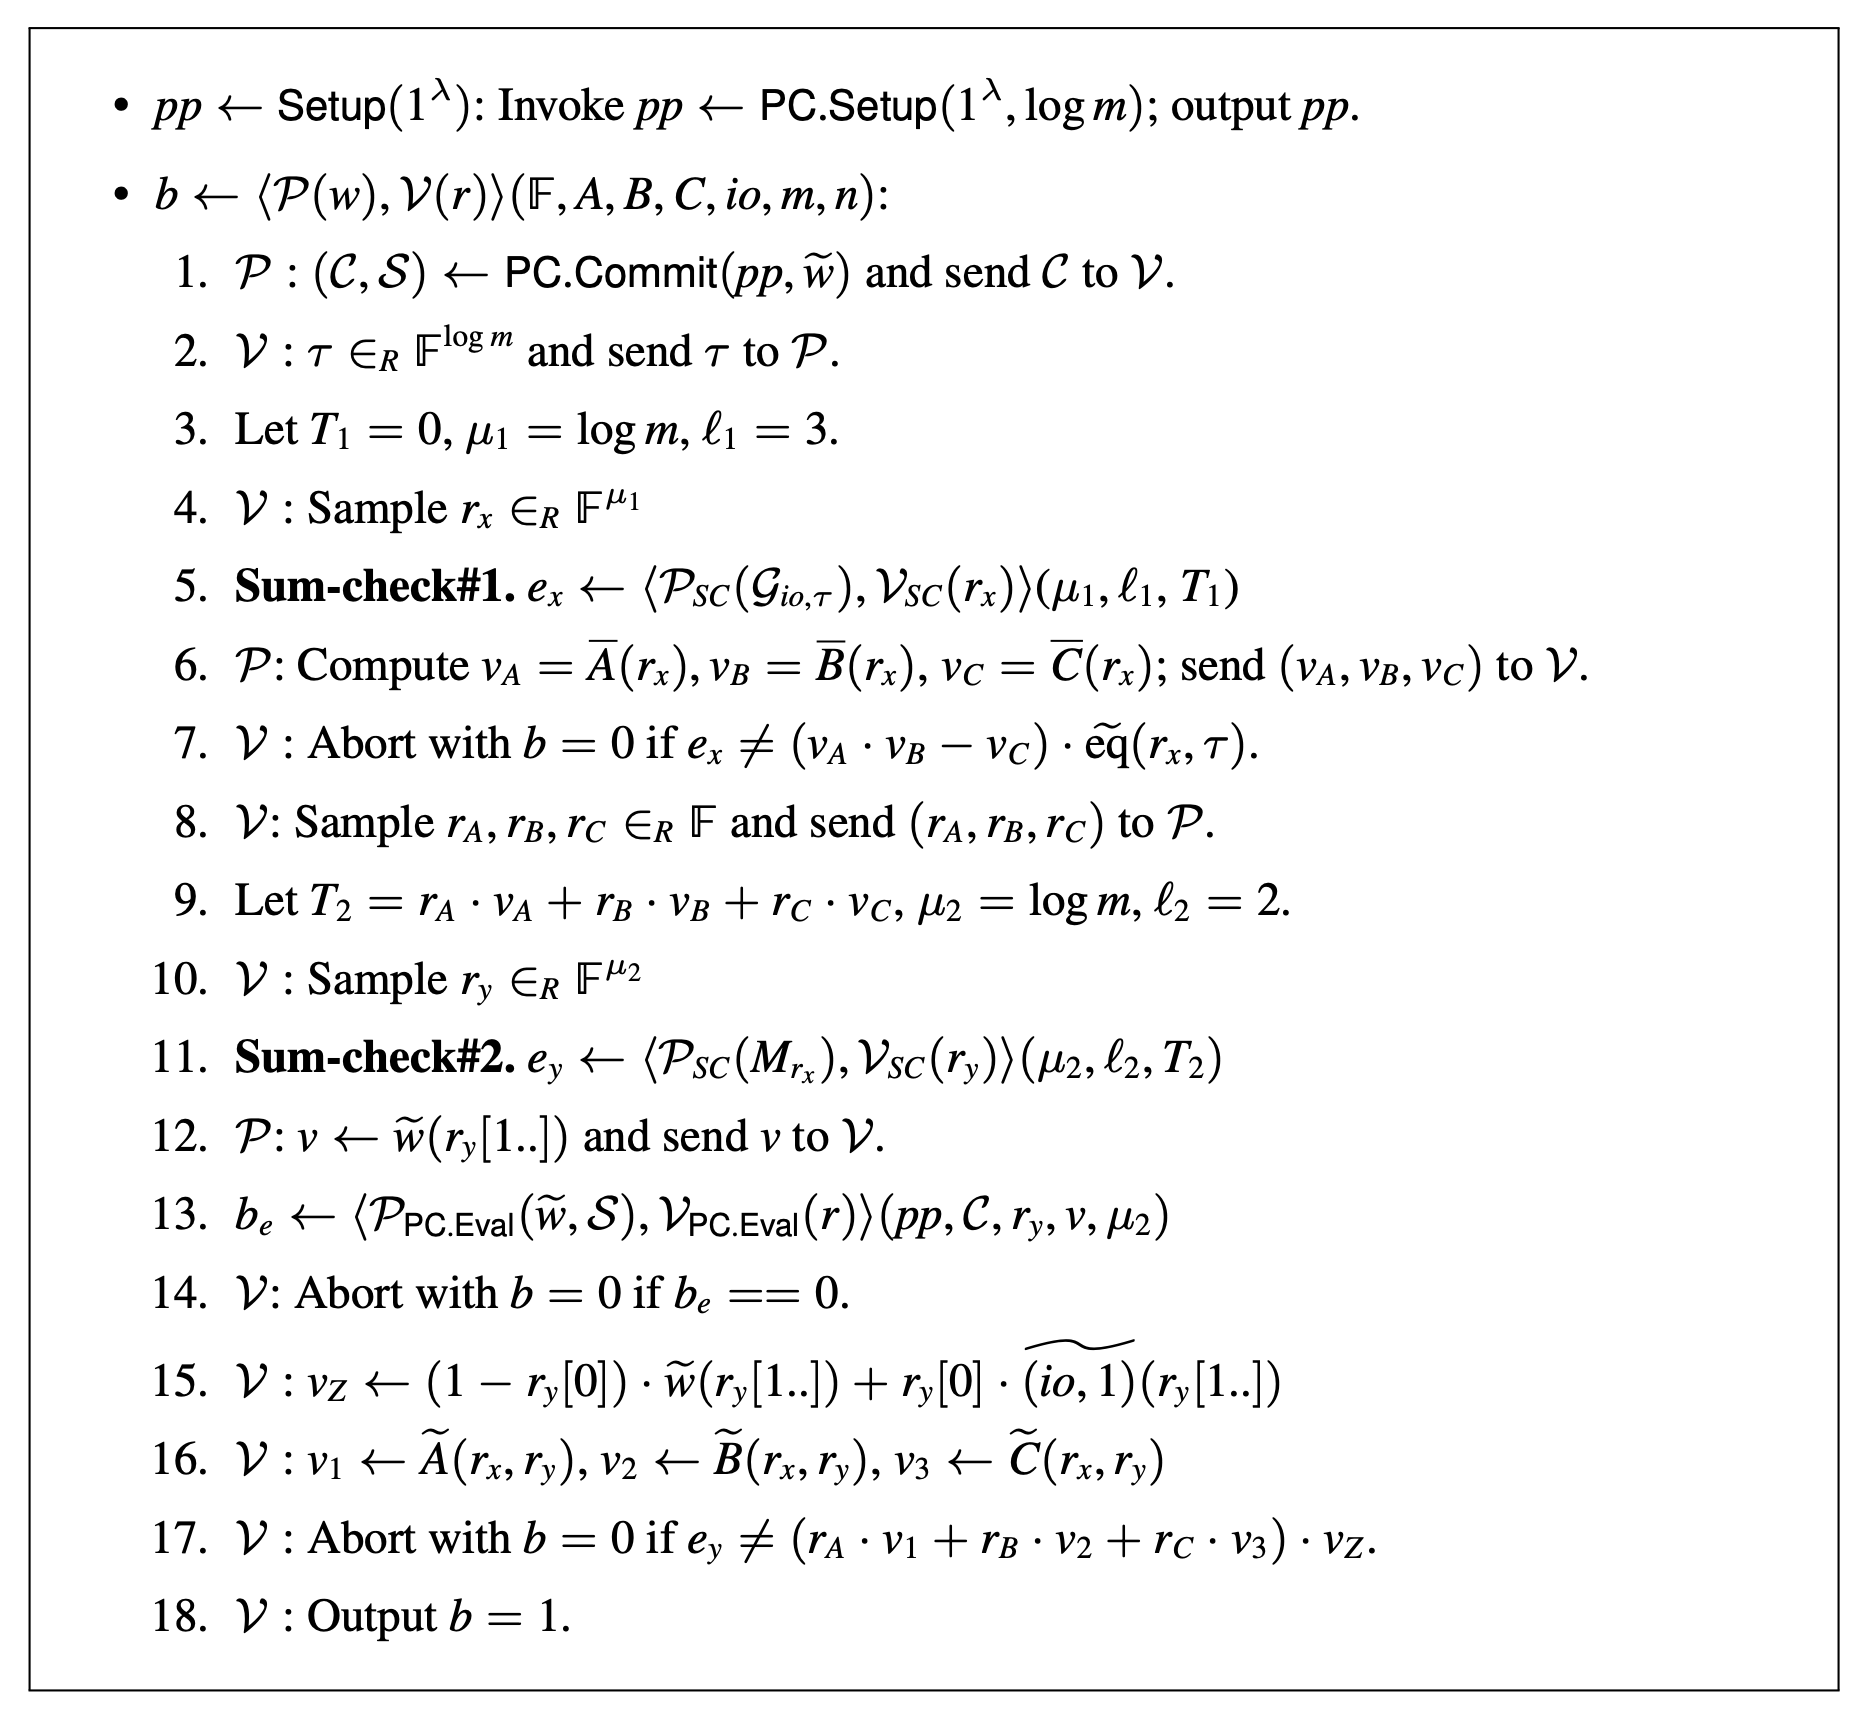
\includegraphics{figures/spartan-description.png}
    \caption{The Spartan protocol description, from the original paper.}
    \label{fig:spartan_protocol}
\end{figure}

After stripping away the polynomial commitment scheme, the protocol has the following structure:

\begin{description}
    \item[Setup:] This step is part of the polynomial commitment scheme and is not part of the PIOP we formalize.
    \item[Interaction:] The interaction is between a prover $\mathcal{P}$ with witness $w$ and a verifier $\mathcal{V}$ with public inputs $(\mathbb{F}, A, B, C, \text{io}, m, n)$.
    \begin{enumerate}
        \item $\mathcal{P}$: Sends oracle access to the multilinear extension of the witness, $\tilde{w}$, to $\mathcal{V}$. In the original paper, this is a commitment $(C,S) \leftarrow \text{PC.Commit}(\text{pp}, \tilde{w})$.
        \item $\mathcal{V}$: Samples a random challenge $\tau \in \mathbb{F}^{\log m}$ and sends it to $\mathcal{P}$.
        \item Let $T_1 = 0$, $\mu_1 = \log m$, $\ell_1 = 3$. These are parameters for the first sum-check protocol.
        \item $\mathcal{V}$: Samples a random challenge $r_x \in \mathbb{F}^{\mu_1}$.
        \item \textbf{Sum-check\#1.} A sum-check protocol is executed. The verifier receives the claimed evaluation $e_x$. The prover of the sum-check has oracle access to a polynomial $G_{io, \tau}$, and the verifier has oracle access to $r_x$. The parameters for this sub-protocol are $(\mu_1, \ell_1, T_1)$.
        \item $\mathcal{P}$: Computes evaluations $v_A = \tilde{A}(r_x)$, $v_B = \tilde{B}(r_x)$, $v_C = \tilde{C}(r_x)$ and sends them to $\mathcal{V}$. $\tilde{A}, \tilde{B}, \tilde{C}$ are multilinear extensions of the matrices $A, B, C$.
        \item $\mathcal{V}$: Aborts if $e_x \neq (v_A \cdot v_B - v_C) \cdot \tilde{\text{eq}}(r_x, \tau)$. This is the verifier's check for the first sum-check.
        \item $\mathcal{V}$: Samples random challenges $r_A, r_B, r_C \in \mathbb{F}$ and sends them to $\mathcal{P}$.
        \item Let $T_2 = r_A \cdot v_A + r_B \cdot v_B + r_C \cdot v_C$, $\mu_2 = \log n$, $\ell_2 = 2$. These are parameters for the second sum-check protocol. Note: The image states $\mu_2 = \log m$, which is likely a typo and should be $\log n$.
        \item $\mathcal{V}$: Samples a random challenge $r_y \in \mathbb{F}^{\mu_2}$.
        \item \textbf{Sum-check\#2.} Another sum-check protocol is executed. The verifier receives the claimed evaluation $e_y$.
        \item $\mathcal{P}$: Computes $v \leftarrow \tilde{w}(r_y[1..])$ and sends $v$ to $\mathcal{V}$.
        \item This step involves a polynomial commitment evaluation proof. In our PIOP formalization, this check is not needed as the verifier has direct oracle access to $\tilde{w}$.
        \item $\mathcal{V}$: This step is part of the evaluation proof check, so it is omitted.
        \item $\mathcal{V}$: Computes $v_Z \leftarrow (1 - r_y[0]) \cdot \tilde{w}(r_y[1..]) + r_y[0] \cdot \widetilde{(\text{io}, 1)}(r_y[1..])$. This reconstructs the evaluation of the combined input-witness vector polynomial $\tilde{z}$.
        \item $\mathcal{V}$: Queries oracles for $\tilde{A}, \tilde{B}, \tilde{C}$ at $(r_x, r_y)$ to get $v_1, v_2, v_3$.
        \item $\mathcal{V}$: Aborts if $e_y \neq (r_A \cdot v_1 + r_B \cdot v_2 + r_C \cdot v_3) \cdot v_Z$. This is the final check.
        \item $\mathcal{V}$: Outputs 1.
    \end{enumerate}
\end{description}

\subsection{Formalization using IOR Composition}

We fix an R1CS size with $m$ constraints, $n_x$ public inputs and $n_w$ witness variables, and set
\[
  s = \lceil \log_2 m \rceil, \qquad t = \lceil \log_2 \max(n_x, n_w) \rceil + 1.
\]
The formalized PIOP pads the instance to $2^s$ constraints and to public-input and witness
vectors of length $2^{t-1}$, so that $z = (x, w)$ is indexed by $\{0,1\}^t$. It is the sequential
composition of seven oracle reductions; the bound in brackets is the round-by-round knowledge
error charged to each challenge of that stage, where $q = |\mathbb{F}|$.

\begin{definition}[Spartan PIOP]
    \label{def:spartan_reduction}
    \lean{Spartan.oracleReduction, Spartan.Assembly.stage,
      Spartan.PublicParams.forSize}
    \leanok
    \uses{def:oracle_reduction, def:sendsinglewitness_adapter, def:sumcheck_single_round}
    The Spartan oracle reduction is the composition of:
    \begin{enumerate}
        \item \textbf{Witness attachment} [$0$]: the prover sends the padded witness table as an
        oracle message, an instance of the adapter of Definition~\ref{def:sendsinglewitness_adapter}.
        \item \textbf{Zero-check} [$s/q$]: the verifier samples $\tau \in \mathbb{F}^{s}$, reducing
        the claim that every constraint holds (the multilinear extension of the residual
        $(Az) \circ (Bz) - Cz$ is zero) to the claim that this extension vanishes at $\tau$,
        equivalently
        $\sum_{x \in \{0,1\}^s} \tilde{\text{eq}}(\tau, x)\,((Az)_x (Bz)_x - (Cz)_x) = 0$.
        \item \textbf{First sum-check} [$3/q$]: sum-check of degree $3$ in $s$ rounds, ending at a
        point $r_x$.
        \item \textbf{Send evaluations} [$0$]: the prover sends $v_A, v_B, v_C$, and the verifier
        checks the first sum-check's final claim against them.
        \item \textbf{Batching} [$1/q$]: the verifier samples one challenge consisting of three
        independent coefficients $(r_A, r_B, r_C)$, forming the claim
        $T_2 = r_A v_A + r_B v_B + r_C v_C$.
        \item \textbf{Second sum-check} [$2/q$]: sum-check of degree $2$ in $t$ rounds, ending at
        a point $r_y$.
        \item \textbf{Terminal check} [$0$]: the verifier evaluates the second virtual polynomial at
        $r_y$ through the matrix and witness oracles and compares it with the final claim.
    \end{enumerate}
\end{definition}

\begin{theorem}[Perfect completeness]
    \label{thm:spartan_completeness}
    \lean{Spartan.perfectCompleteness}
    \leanok
    \uses{def:spartan_reduction, thm:sumcheck_perfect_completeness}
    The Spartan oracle reduction is perfectly complete from the original (unpadded) R1CS
    satisfiability relation to the trivial output relation.
\end{theorem}

\begin{theorem}[Round-by-round knowledge soundness]
    \label{thm:spartan_rbr}
    \lean{Spartan.rbrKnowledgeSoundnessWith, Spartan.challengeError}
    \leanok
    \uses{def:spartan_reduction, thm:sumcheck_rbr_knowledge_soundness_standard}
    The Spartan verifier is fixed-prefix round-by-round knowledge sound for the original R1CS
    relation, with each challenge charged the error of its stage listed in
    Definition~\ref{def:spartan_reduction}. The state function is the composition of the stage
    state functions, retaining every earlier rejecting check.
\end{theorem}

\begin{theorem}[Knowledge soundness]
    \label{thm:spartan_knowledge_soundness}
    \lean{Spartan.totalError, Spartan.error_ledger, Spartan.sum_challengeError,
      Spartan.knowledgeSoundnessWith, Spartan.straightlineExtractor,
      Spartan.foldExtractor_eq_straightlineExtractor,
      Spartan.knowledgeSoundnessWith_straightlineExtractor, Spartan.knowledgeSoundness,
      Spartan.knowledgeSoundness_clipped}
    \leanok
    \uses{thm:spartan_rbr, thm:rbr_knowledge_soundness_implies_knowledge_soundness}
    The per-challenge errors sum to
    \[
      \frac{s}{q} + s \cdot \frac{3}{q} + \frac{1}{q} + t \cdot \frac{2}{q} = \frac{4s + 2t + 1}{q}.
    \]
    The Spartan verifier is knowledge sound for the original R1CS relation with error
    $(4s + 2t + 1)/q$, and also with error $\min(1, (4s + 2t + 1)/q)$. The extractor obtained by
    folding the round-by-round extractors equals an executable straight-line extractor, which
    restricts the first message (the padded witness table) to the original witness coordinates.
\end{theorem}
